%!TEX root = ../../../super_main.tex

\section{\emph{Launcher} Grid Settings}
\label{sec:launcher_grid_setting}
%% Indsæt reference til usability report
We fixed a usability problem in the \launcher settings (see \figref{fig:launcher_grid_settings_old}) by changing the description of grid settings. The title before read \translated{Gitterstørrelse}{Grid size}, and the old description read \translated{Indstil størrelsen på gitteret for hjemmeskærmen}{Set the size of the grid for the home screen}. The new title reads \translated{Antal Apps}{Number of Apps}, and the new description reads \translated{Indstil antallet af apps for hjemmeskærmen}{Set the number of apps for the home screen}.

The users had trouble figuring what moving the slider meant. Did moving the slider to the right result in more or less applications in the main screen of the launcher? We changed to text to indicate the number of applications instead of the grid size. The result can be seen in \figref{fig:launcher_grid_settings_new}. 

\begin{figure}[!htbp]
    \centering

    \begin{subfigure}[t]{0.75\textwidth}
        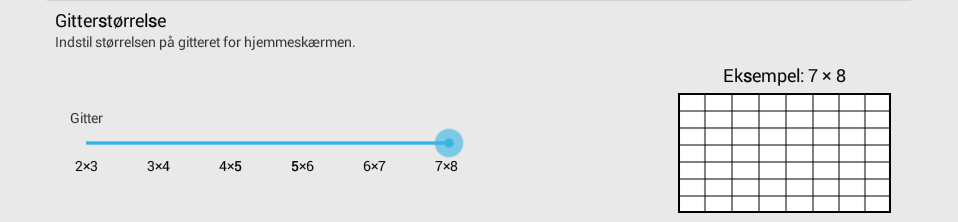
\includegraphics[width=\textwidth]{sprint_four/grid_setting_before}
        \caption{Grid setting before}
        \label{fig:launcher_grid_settings_old}
        \vspace*{1cm}
    \end{subfigure}
    \begin{subfigure}[t]{0.75\textwidth}
        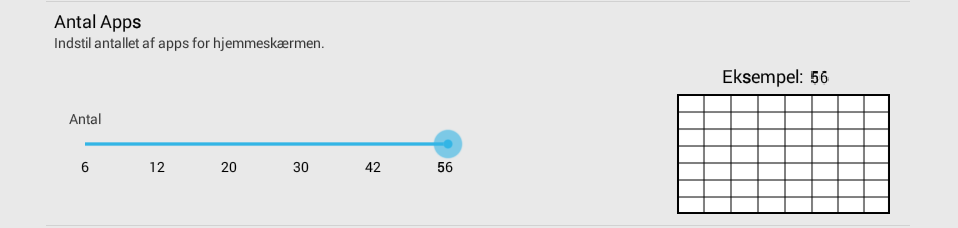
\includegraphics[width=\textwidth]{sprint_four/grid_setting_after}
        \caption{Grid setting after}
        \label{fig:launcher_grid_settings_new}
    \end{subfigure}
    
    \caption{Launcher grid settings before and after}
    \label{fig:launcher_grid_settings}
\end{figure}